\documentclass[11pt]{article}

\usepackage[utf8]{inputenc}
\usepackage[T1]{fontenc}
\usepackage[spanish]{babel}
\usepackage{lmodern}
\usepackage[margin=2.5cm]{geometry}
\usepackage{graphicx}
\usepackage{booktabs}
\usepackage{amsmath}
\usepackage{listings}
\usepackage{xcolor}
\usepackage{float}
\usepackage{url}
\usepackage[hidelinks]{hyperref}

\lstset{
  language=C++,
  basicstyle=\ttfamily\small,
  keywordstyle=\color{blue}\bfseries,
  commentstyle=\color{gray}\itshape,
  backgroundcolor=\color{gray!8},
  numbers=left,
  numberstyle=\tiny,
  breaklines=true,
  showstringspaces=false,
  captionpos=b
}
\renewcommand{\lstlistingname}{Código}

\title{Laboratorio 2\\
Evaluación del desempeño de algoritmos y comportamiento de la memoria caché}
\author{[Nombre del estudiante]\\Universidad Nacional de San Agustín de Arequipa}
\date{\today}

\begin{document}
\maketitle

%============================================================
\section{Introducción}

La complejidad de un algoritmo indica cuántas operaciones hace, pero no
cuánto tarda cada operación. En la práctica, leer un dato que ya está en la
memoria caché es mucho más rápido que traerlo desde la memoria principal
(RAM). Por eso, dos programas con la misma complejidad pueden tardar tiempos
muy distintos.

El objetivo de este laboratorio es comprobarlo con experimentos. Se
compararon algoritmos que hacen el mismo número de operaciones pero acceden a
la memoria en distinto orden: los dos pares de bucles anidados del libro de
Pacheco, la multiplicación clásica de matrices y la multiplicación por
bloques. Se midieron los tiempos en dos computadoras con distinto tamaño de
caché y se usó Valgrind (Cachegrind) para contar los fallos de caché.

Los resultados muestran que recorrer una matriz por columnas fue hasta 20
veces más lento que por filas, y que la multiplicación por bloques fue hasta
10,9 veces más rápida que la clásica. En ambos casos la complejidad es la
misma; la diferencia se debe a la memoria caché.

%============================================================
\section{Entorno y forma de medir}

Se usaron dos computadoras. En ambas los programas se ejecutaron dentro de
una máquina virtual con Lubuntu.

\begin{table}[H]
\centering
\caption{Equipos utilizados.}
\begin{tabular}{lll}
\toprule
 & \textbf{Laptop} & \textbf{PC} \\
\midrule
Procesador & Intel i5-3230M & Intel i5-10400 \\
Caché L1 (datos) & 32 KB & 32 KB \\
Caché L2 & 256 KB & 256 KB \\
Caché L3 & \textbf{3 MB} & \textbf{12 MB} \\
Sistema & \multicolumn{2}{c}{Lubuntu 16.04 (32 bits) en VMware} \\
Compilador & \multicolumn{2}{c}{g++ 5.4.0 con \texttt{-std=c++14 -O2 -g}} \\
Valgrind & \multicolumn{2}{c}{3.11.0} \\
\bottomrule
\end{tabular}
\end{table}

\begin{itemize}
\item El tiempo se mide con \texttt{std::chrono} solo alrededor de los bucles.
\item Cada caso se ejecutó 3 veces y se usa el promedio.
\item Las matrices se guardan en un \texttt{vector} fila por fila: el elemento
      $(i,j)$ está en la posición \texttt{i*n + j}.
\item Como se midió dentro de máquinas virtuales, los tiempos pueden tener
      algo de ruido, sobre todo los más pequeños.
\end{itemize}

%============================================================
\section{Actividad 1: bucles anidados}

\subsection{Código}

Se implementaron los dos pares de bucles del libro de Pacheco~\cite{pacheco}
(capítulo 2, página 22). Los dos calculan $y = A \cdot x$.

\begin{lstlisting}[caption={Primer par: recorre la matriz por filas.}]
for (int i = 0; i < MAX; i++)
    for (int j = 0; j < MAX; j++)
        y[i] += A[i * MAX + j] * x[j];
\end{lstlisting}

\begin{lstlisting}[caption={Segundo par: recorre la matriz por columnas.}]
for (int j = 0; j < MAX; j++)
    for (int i = 0; i < MAX; i++)
        y[i] += A[i * MAX + j] * x[j];
\end{lstlisting}

La única diferencia es el orden de los bucles: en el primero va primero
\texttt{i} y en el segundo va primero \texttt{j}.

\subsection{Iteraciones y complejidad}

En los dos casos el bucle de afuera da \texttt{MAX} vueltas y, por cada una,
el de adentro da otras \texttt{MAX}. Entonces la línea de adentro se ejecuta
\[
\texttt{MAX} \times \texttt{MAX} = \texttt{MAX}^2 \text{ veces.}
\]
Los dos pares tienen la misma complejidad: $O(\texttt{MAX}^2)$.

\subsection{Resultados}

\begin{table}[H]
\centering
\caption{Tiempos en segundos. ``Veces'' indica cuántas veces es más lento el recorrido por columnas.}
\small
\begin{tabular}{rrr|rrr|rrr}
\toprule
 & & & \multicolumn{3}{c|}{\textbf{Laptop}} & \multicolumn{3}{c}{\textbf{PC}} \\
MAX & Iteraciones & Tamaño de $A$ & Filas & Columnas & Veces & Filas & Columnas & Veces \\
\midrule
500  & 250\,000    & 1,9 MB  & 0,0003 & 0,0006 & 2,0  & 0,0003 & 0,0003 & 1,0 \\
1000 & 1\,000\,000  & 7,6 MB  & 0,0016 & 0,0188 & 11,6 & 0,0013 & 0,0031 & 2,4 \\
2000 & 4\,000\,000  & 30,5 MB & 0,0077 & 0,0841 & 11,0 & 0,0050 & 0,0347 & 6,9 \\
3000 & 9\,000\,000  & 68,7 MB & 0,0118 & 0,2053 & 17,4 & 0,0110 & 0,0872 & 7,9 \\
4000 & 16\,000\,000 & 122 MB  & 0,0199 & 0,4037 & \textbf{20,2} & 0,0195 & 0,1704 & \textbf{8,7} \\
\bottomrule
\end{tabular}
\end{table}

\begin{figure}[H]
\centering
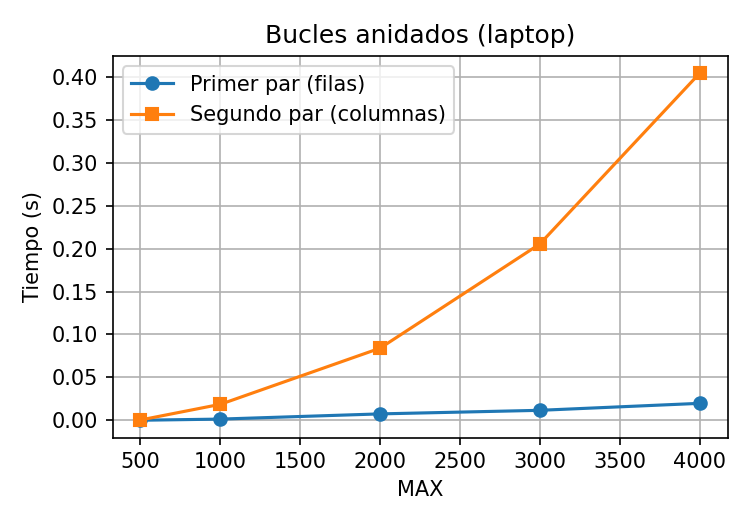
\includegraphics[width=0.48\textwidth]{../graficas/laptop_bucles.png}
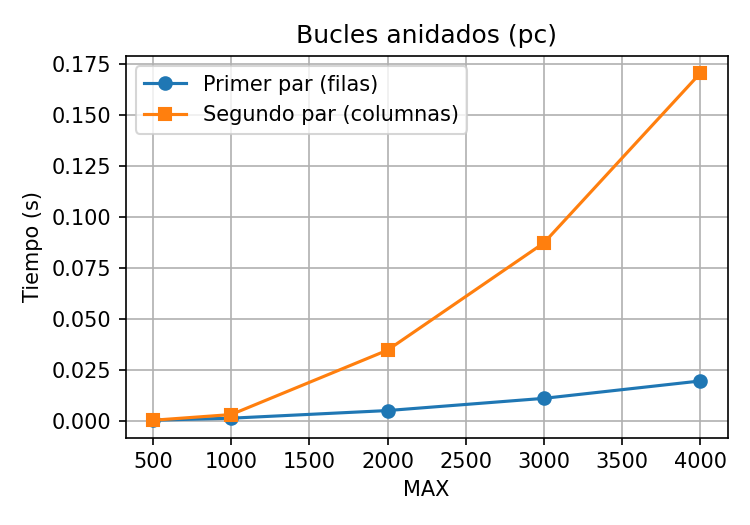
\includegraphics[width=0.48\textwidth]{../graficas/pc_bucles.png}
\caption{Tiempo de los dos pares de bucles: laptop (izquierda) y PC (derecha).}
\end{figure}

\subsection{Análisis}

\begin{itemize}
\item Los dos pares hacen las mismas iteraciones, pero \textbf{por columnas es
      mucho más lento}: hasta 20 veces en la laptop y 8,7 veces en la PC.
\item La diferencia crece cuando la matriz ya no cabe en la caché L3. En la
      laptop (L3 de 3 MB) el salto ocurre entre \texttt{MAX} = 500 (1,9 MB) y
      1000 (7,6 MB). En la PC (L3 de 12 MB) el salto aparece después, en
      \texttt{MAX} = 2000.
\item La razón se explica en la actividad 4: la matriz está guardada por filas,
      así que recorrerla por filas aprovecha la caché y por columnas no.
\end{itemize}

%============================================================
\section{Actividad 2: multiplicación clásica}

\subsection{Código}

\begin{lstlisting}[caption={Multiplicación clásica con tres bucles.}]
for (int i = 0; i < n; i++)
    for (int j = 0; j < n; j++)
        for (int k = 0; k < n; k++)
            C[i * n + j] += A[i * n + k] * B[k * n + j];
\end{lstlisting}

\subsection{Complejidad}

Hay tres bucles de $n$ vueltas, uno dentro de otro, así que la línea de adentro
se ejecuta $n \times n \times n = n^3$ veces. La complejidad es $O(n^3)$.

Esto significa que si $n$ se duplica, el tiempo debería multiplicarse por
$2^3 = 8$.

\subsection{Resultados}

\begin{table}[H]
\centering
\caption{Tiempo de la multiplicación clásica (segundos).}
\begin{tabular}{rrr}
\toprule
$n$ & Laptop & PC \\
\midrule
100  & 0,0013  & 0,0009 \\
200  & 0,0130  & 0,0082 \\
300  & 0,0417  & 0,0279 \\
400  & 0,1340  & 0,0696 \\
500  & 0,3578  & 0,1303 \\
600  & 2,6466  & 0,2300 \\
800  & 9,5086  & 0,6100 \\
1000 & 16,2976 & 2,8045 \\
\bottomrule
\end{tabular}
\end{table}

\begin{figure}[H]
\centering
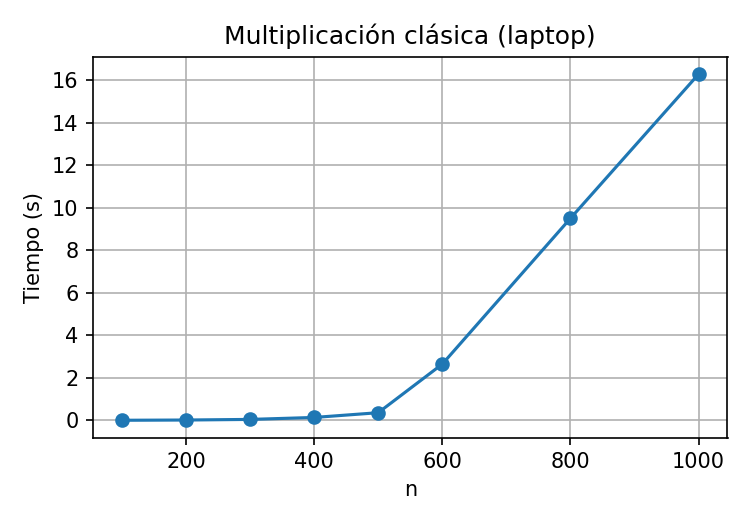
\includegraphics[width=0.48\textwidth]{../graficas/laptop_clasica.png}
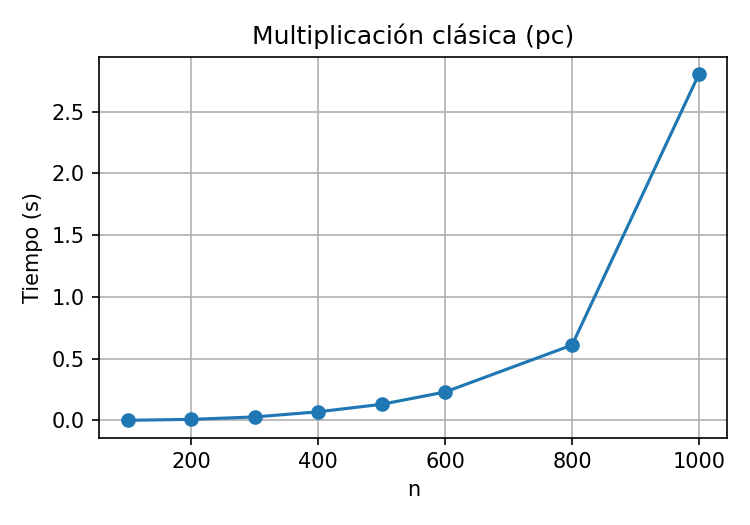
\includegraphics[width=0.48\textwidth]{../graficas/pc_clasica.png}
\caption{Tiempo de la multiplicación clásica: laptop (izquierda) y PC (derecha).}
\end{figure}

\subsection{Análisis}

\begin{itemize}
\item Al pasar de $n=500$ a $n=1000$ (el doble), el tiempo debería
      multiplicarse por 8, pero en la laptop se multiplicó por \textbf{45,5}
      y en la PC por \textbf{21,5}.
\item En la laptop hay un salto muy grande entre $n=500$ y $n=600$: el tiempo
      sube 7,4 veces aunque $n$ solo aumentó un 20\,\%. En la PC el salto
      aparece más tarde, entre $n=800$ y $n=1000$, porque tiene más caché.
\item El algoritmo sigue haciendo $n^3$ operaciones. Lo que cambia es que,
      cuando las matrices ya no caben en la caché, cada operación tarda más
      porque hay que ir a buscar los datos a la RAM.
\end{itemize}

%============================================================
\section{Actividad 3: multiplicación por bloques}

\subsection{Fundamento}

La idea es dividir cada matriz en pedazos pequeños (bloques) de $b \times b$
y multiplicar bloque por bloque. Se hacen exactamente las mismas operaciones
que en la clásica, pero en otro orden.

La ventaja es que un bloque pequeño cabe completo en la caché. Mientras se
trabaja con un bloque, casi todos los datos que se necesitan ya están
cargados, y se evitan viajes a la RAM.

\subsection{Código}

\begin{lstlisting}[caption={Multiplicación por bloques con seis bucles.}]
for (int ii = 0; ii < n; ii += b)          // bloque de filas
    for (int jj = 0; jj < n; jj += b)      // bloque de columnas
        for (int kk = 0; kk < n; kk += b)  // bloque intermedio
            for (int i = ii; i < min(ii + b, n); i++)
                for (int j = jj; j < min(jj + b, n); j++)
                    for (int k = kk; k < min(kk + b, n); k++)
                        C[i * n + j] += A[i * n + k] * B[k * n + j];
\end{lstlisting}

Los tres primeros bucles eligen el bloque y los tres últimos multiplican
dentro del bloque. El \texttt{min} evita salirse de la matriz cuando $n$ no es
múltiplo de $b$.

Para comprobar que el resultado es correcto, el programa
\texttt{verificar.cpp} compara elemento por elemento el resultado con el de la
multiplicación clásica, usando $n=500$ y $b=32$. Se eligió ese caso porque
500 no es múltiplo de 32 y el último bloque queda incompleto (20 filas). Los
dos resultados fueron idénticos.

\textbf{Complejidad:} sigue siendo $O(n^3)$, porque se hacen las mismas $n^3$
multiplicaciones.

\subsection{Resultados}

Se probaron bloques de 16, 32, 64 y 128. Entre paréntesis se indica cuántas
veces es más rápida que la clásica.

\begin{table}[H]
\centering
\caption{Tiempo (s) de la multiplicación por bloques.}
\small
\begin{tabular}{llrrrrr}
\toprule
Equipo & $n$ & Clásica & $b=16$ & $b=32$ & $b=64$ & $b=128$ \\
\midrule
Laptop & 500  & 0,358  & 0,180 (2,0×) & 0,191 (1,9×) & 0,183 (2,0×) & 0,188 (1,9×) \\
Laptop & 800  & 9,509  & 1,112 (8,5×) & 1,155 (8,2×) & \textbf{0,888 (10,7×)} & 0,925 (10,3×) \\
Laptop & 1000 & 16,298 & 2,019 (8,1×) & \textbf{1,495 (10,9×)} & 1,522 (10,7×) & 1,738 (9,4×) \\
\midrule
PC & 500  & 0,130 & 0,110 (1,2×) & \textbf{0,108 (1,2×)} & 0,114 (1,1×) & 0,126 (1,0×) \\
PC & 800  & 0,610 & \textbf{0,500 (1,2×)} & 0,533 (1,1×) & 0,541 (1,1×) & 0,569 (1,1×) \\
PC & 1000 & 2,805 & 0,934 (3,0×) & \textbf{0,908 (3,1×)} & 0,960 (2,9×) & 1,033 (2,7×) \\
\bottomrule
\end{tabular}
\end{table}

\begin{figure}[H]
\centering
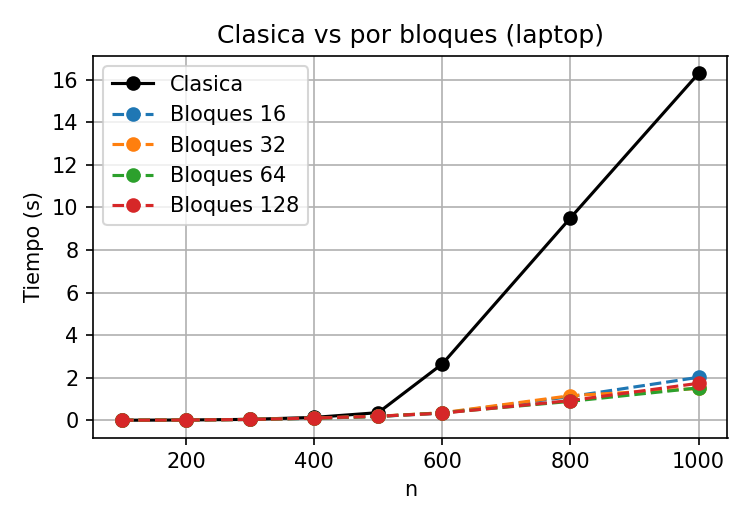
\includegraphics[width=0.48\textwidth]{../graficas/laptop_clasica_vs_bloques.png}
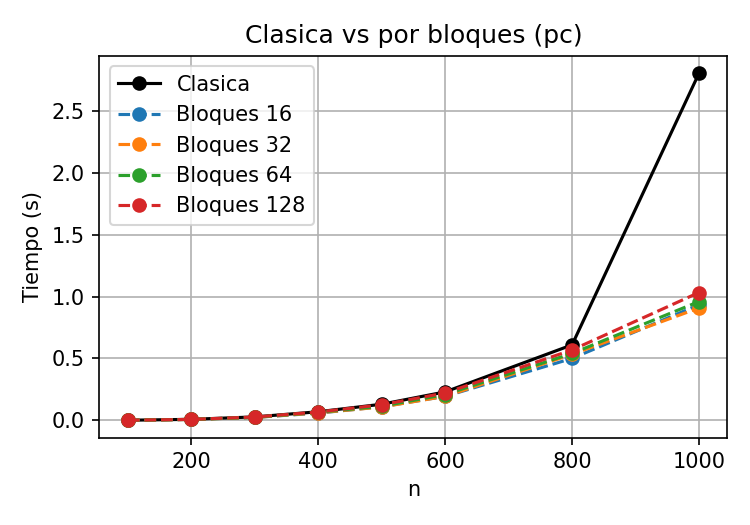
\includegraphics[width=0.48\textwidth]{../graficas/pc_clasica_vs_bloques.png}
\caption{Clásica frente a bloques: laptop (izquierda) y PC (derecha).}
\end{figure}

\begin{figure}[H]
\centering
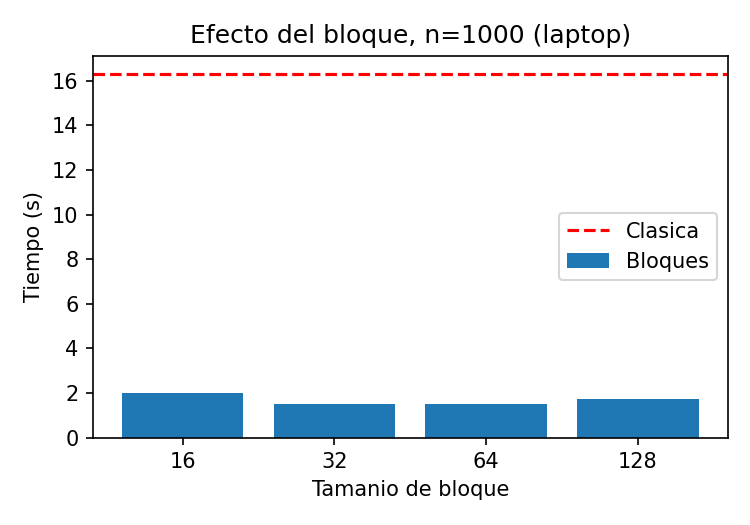
\includegraphics[width=0.48\textwidth]{../graficas/laptop_tam_bloque.png}
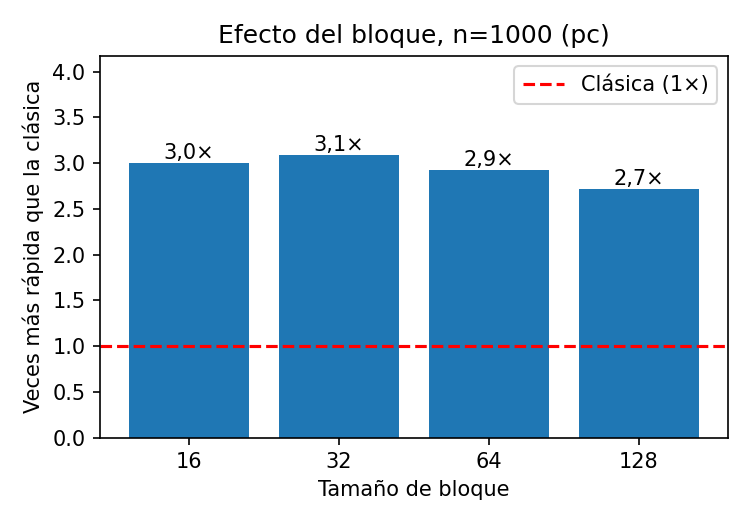
\includegraphics[width=0.48\textwidth]{../graficas/pc_tam_bloque.png}
\caption{Cuántas veces es más rápida la versión por bloques que la clásica con
$n=1000$, según el tamaño de bloque. La línea roja (1×) representa la clásica.}
\end{figure}

\subsection{Análisis}

\begin{itemize}
\item Con matrices pequeñas casi no hay diferencia, porque todo cabe en la caché.
\item Con matrices grandes la versión por bloques es mucho más rápida: con
      $n=1000$, \textbf{10,9 veces} en la laptop (16,3 s contra 1,5 s) y
      \textbf{3,1 veces} en la PC.
\item \textbf{Tamaño de bloque:} se necesitan 3 bloques a la vez ($A$, $B$ y
      $C$), cada uno de $b \times b$ números de 8 bytes. Para que quepan en la
      caché L1 de 32 KB:
      \[
      3 \times b^2 \times 8 \le 32\,768 \quad\Rightarrow\quad b \le 36
      \]
      Por eso se esperaba que $b=32$ fuera bueno, y así fue: es el mejor para
      $n=1000$ en los dos equipos. Con $b=128$ el bloque ya no cabe en L1 y el
      tiempo empeora.
\end{itemize}

\textbf{¿Por qué es más rápida si tiene la misma complejidad?} Porque la
complejidad solo cuenta operaciones, no cuánto tarda cada una. La versión por
bloques hace las mismas operaciones, pero con los datos casi siempre en la
caché, así que cada operación es más rápida.

%============================================================
\section{Actividad 4: movimiento de datos y memoria caché}

\subsection{Cómo se accede a los elementos}

La memoria es una fila larga de posiciones, y la matriz se guarda fila por
fila. Por ejemplo, una matriz de $3 \times 3$ queda así en memoria:

\begin{center}
\ttfamily
\begin{tabular}{|c|c|c|c|c|c|c|c|c|}
\hline
a00 & a01 & a02 & a10 & a11 & a12 & a20 & a21 & a22 \\
\hline
0 & 1 & 2 & 3 & 4 & 5 & 6 & 7 & 8 \\
\hline
\end{tabular}
\end{center}

\begin{itemize}
\item \textbf{Por filas} se visitan las posiciones 0, 1, 2, 3, 4\dots{}: siempre
      la de al lado.
\item \textbf{Por columnas} se visitan 0, 3, 6, 1, 4, 7\dots{}: se salta de $n$
      en $n$.
\end{itemize}

La caché no carga un dato suelto, sino un pedazo de 64 bytes (8 números
\texttt{double}). Al recorrer por filas, los siguientes 7 datos ya vienen
cargados. Al recorrer por columnas, cada acceso cae en otro pedazo y casi
siempre hay un fallo de caché.

En la \textbf{multiplicación clásica}, \texttt{A[i*n+k]} se recorre por filas
(bien), pero \texttt{B[k*n+j]} se recorre por columnas (mal). En la
\textbf{multiplicación por bloques} el acceso a $B$ sigue siendo por columnas,
pero solo dentro de un bloque pequeño que cabe en la caché.

\subsection{Localidad espacial y temporal}

\begin{itemize}
\item \textbf{Localidad espacial:} si se usa un dato, probablemente se usarán
      pronto los que están a su lado. Recorrer por filas aprovecha esto;
      recorrer por columnas no.
\item \textbf{Localidad temporal:} si se usa un dato, probablemente se volverá
      a usar pronto. En la clásica, los datos de $B$ se vuelven a usar, pero
      pasa tanto tiempo que la caché ya los borró. Los bloques hacen que se
      vuelvan a usar enseguida, mientras siguen en la caché.
\end{itemize}

\subsection{Costo del movimiento de datos}

La memoria está organizada en niveles: mientras más cerca del procesador, más
rápida pero más pequeña. Los tiempos aproximados de acceso son~\cite{hennessy}:

\begin{table}[H]
\centering
\caption{Jerarquía de memoria (valores aproximados).}
\begin{tabular}{lrr}
\toprule
Nivel & Tamaño (laptop) & Tiempo de acceso aprox. \\
\midrule
Caché L1 & 32 KB  & $\sim$1 ns \\
Caché L2 & 256 KB & $\sim$4 ns \\
Caché L3 & 3 MB   & $\sim$10--40 ns \\
RAM      & 2 GB   & $\sim$100 ns \\
\bottomrule
\end{tabular}
\end{table}

Un fallo de caché que obliga a ir a la RAM puede costar 100 veces más que
leer desde L1. Por eso, aunque el algoritmo tenga la misma complejidad, el
tiempo real depende mucho de cuántos fallos tenga:
\[
\text{tiempo} \approx \text{operaciones} \times \text{costo de operar} +
\text{fallos de caché} \times \text{costo de cada fallo}
\]
Esto se ve en los datos de la laptop: en la clásica con $n=500$ cada
operación tarda en promedio $0{,}358 / 500^3 \approx 2{,}9$ ns, pero con
$n=1000$ tarda $16{,}3 / 1000^3 \approx 16{,}3$ ns, más de 5 veces más.

%============================================================
\section{Actividad 5: Valgrind y KCachegrind}

\subsection{Cómo se ejecutó}

Se usó Cachegrind indicando el tamaño real de la caché de cada equipo
(script \texttt{cachegrind.sh}):

\begin{lstlisting}[language=bash,numbers=none]
valgrind --tool=cachegrind --I1=32768,8,64 --D1=32768,8,64 \
         --LL=3145728,12,64 ./clasica 500      # laptop
valgrind --tool=cachegrind --I1=32768,8,64 --D1=32768,8,64 \
         --LL=12582912,12,64 ./clasica 500     # PC
\end{lstlisting}

Cachegrind simula dos niveles de caché: el primero (I1 para instrucciones y D1
para datos) y el último (LL, que equivale a L3). No simula L2.

Cada opción recibe tres números: tamaño en bytes, asociatividad (vías) y
tamaño de línea. La L3 de la PC tiene 16 vías, pero Cachegrind exige que el
número de conjuntos sea potencia de 2 y con 16 no se cumple, así que se usaron
12 vías manteniendo los 12 MB. El tamaño es lo que decide si las matrices
caben o no en la caché.

\subsection{Resultados}

\begin{table}[H]
\centering
\caption{Métricas de Cachegrind con $n=500$ y bloque $b=32$.}
\begin{tabular}{lrr}
\toprule
Métrica & Clásica & Bloques \\
\midrule
Instrucciones ejecutadas (I refs)      & 1\,009\,405\,597 & 1\,078\,492\,459 \\
Fallos caché instrucciones I1          & 1\,790 & 1\,783 \\
Fallos caché instrucciones LLi         & 1\,747 & 1\,739 \\
Accesos a memoria de datos (D refs)    & 378\,448\,323 & 412\,112\,074 \\
Fallos caché de datos D1               & \textbf{113\,082\,929} & \textbf{1\,866\,176} \\
Tasa de fallos D1                      & 29,9\,\% & 0,5\,\% \\
Fallos caché de datos LLd (laptop)     & 234\,444 & 237\,388 \\
Fallos caché de datos LLd (PC)         & 100\,160 & 100\,162 \\
\bottomrule
\end{tabular}
\end{table}

Las instrucciones, los accesos y los fallos D1 salieron iguales en los dos
equipos porque tienen la misma caché L1. Solo cambian los fallos LLd, porque
la L3 es distinta.

\begin{figure}[H]
\centering
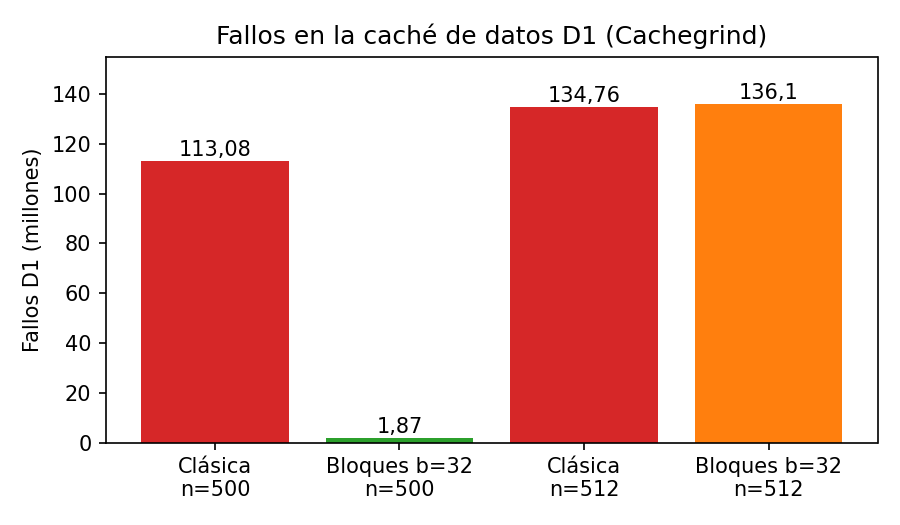
\includegraphics[width=0.65\textwidth]{../graficas/cachegrind_fallos_d1.png}
\caption{Fallos en la caché de datos D1.}
\end{figure}

\textbf{Un resultado inesperado con $n=512$.} Al principio se probó con
$n=512$ y los bloques casi no redujeron los fallos D1 (de 134,8 a 136,1
millones). La causa es que 512 es potencia de 2: los elementos de una columna
de $B$ quedan separados justo 4096 bytes, y todos caen en el mismo grupo
(conjunto) de la caché L1, que solo tiene espacio para 8 pedazos. Se expulsan
entre ellos aunque haya espacio libre en otros grupos. Con $n=500$ esto no
pasa, por eso se usó ese tamaño para la comparación.

\subsection{KCachegrind}

Los archivos generados se abren con:

\begin{lstlisting}[language=bash,numbers=none]
kcachegrind cachegrind/extra_clasica_500.out
kcachegrind cachegrind/extra_bloques_500_32.out
\end{lstlisting}

Se eligió el evento \texttt{L1 Data Read Miss} (fallos de lectura en D1), la
función \texttt{main} y la pestaña \texttt{Source Code}, que muestra cuántos
fallos produce cada línea del código.

\begin{figure}[H]
\centering
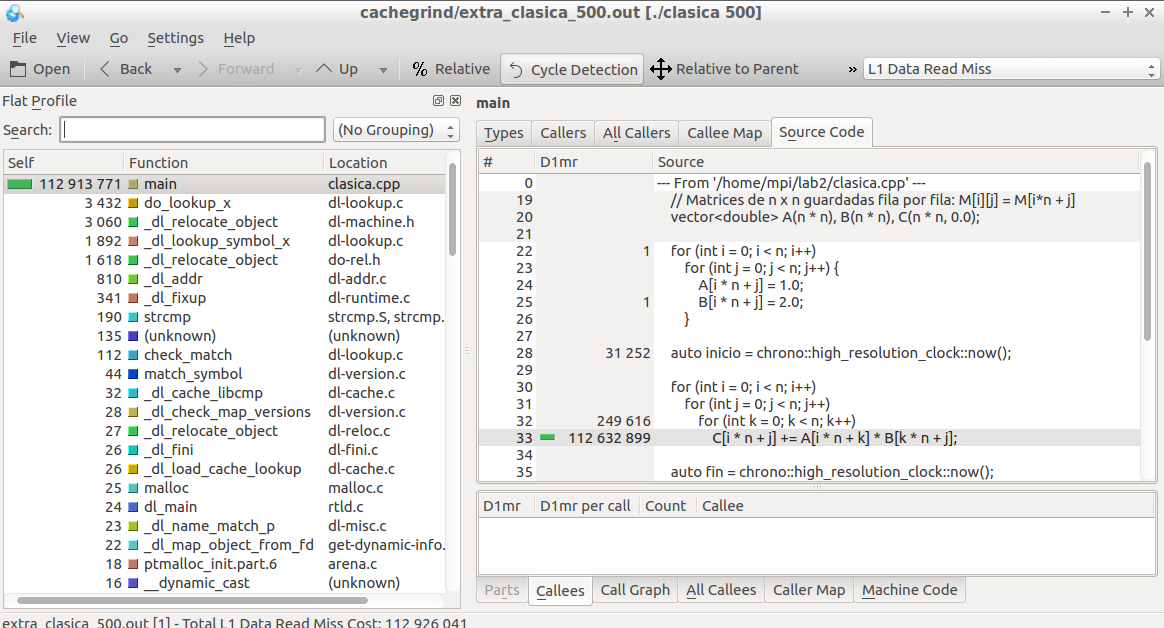
\includegraphics[width=\textwidth]{../graficas/kcachegrind_clasica_500.png}
\caption{KCachegrind, multiplicación clásica ($n=500$): la línea 33 tiene
112\,632\,899 fallos de lectura en D1.}
\end{figure}

\begin{figure}[H]
\centering
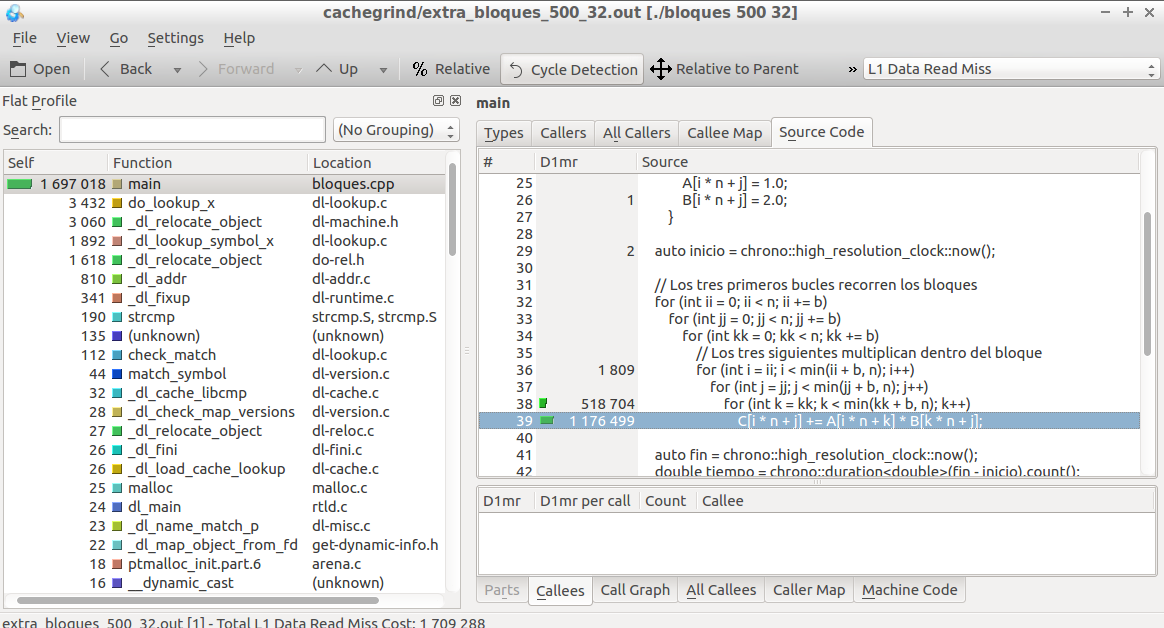
\includegraphics[width=\textwidth]{../graficas/kcachegrind_bloques_500.png}
\caption{KCachegrind, multiplicación por bloques ($n=500$, $b=32$): la misma
operación (línea 39) tiene solo 1\,176\,499 fallos.}
\end{figure}

En las capturas se ve que:
\begin{itemize}
\item En la clásica, la línea \texttt{C[i*n+j] += A[i*n+k] * B[k*n+j];}
      concentra casi todos los fallos: \textbf{112,6 millones} de los 112,9
      millones del programa (99,7\,\%).
\item En la versión por bloques, la misma operación tiene solo
      \textbf{1,2 millones}, unas \textbf{96 veces menos}.
\end{itemize}

\textbf{Último nivel de caché (L3).} También se revisó el evento
\texttt{LL Data Read Miss} (fallos de lectura en el último nivel) para la
clásica con $n=500$ en los dos equipos:

\begin{figure}[H]
\centering
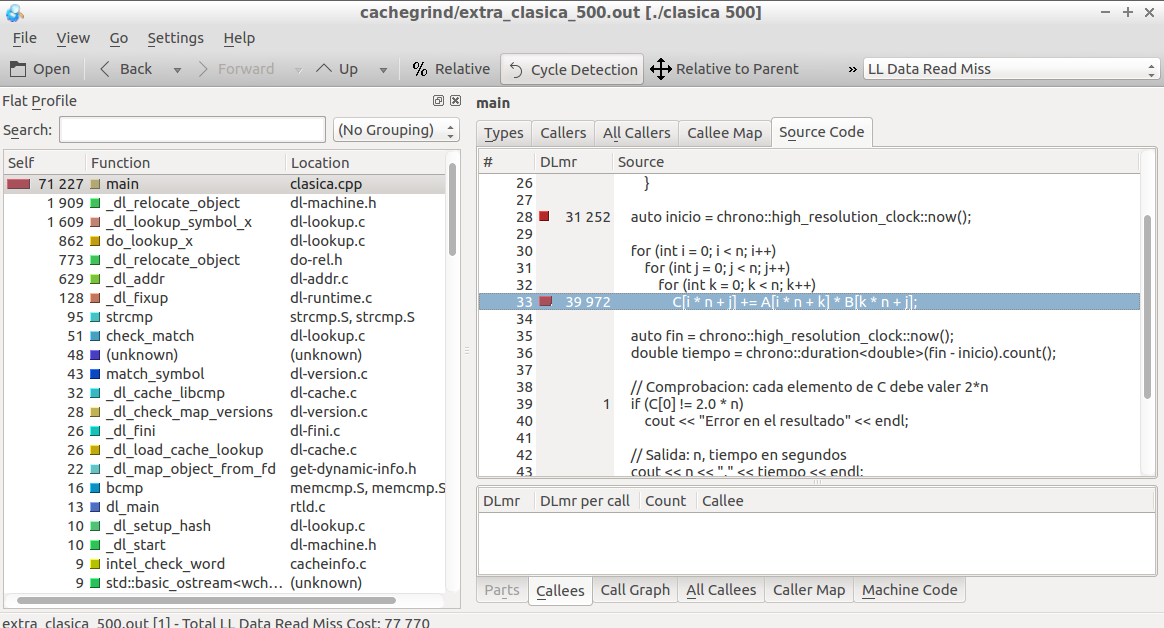
\includegraphics[width=\textwidth]{../graficas/kcachegrind_ll_laptop.png}
\caption{Laptop (L3 de 3 MB), clásica $n=500$: la línea 33 tiene 39\,972
fallos de lectura en el último nivel.}
\end{figure}

\begin{figure}[H]
\centering
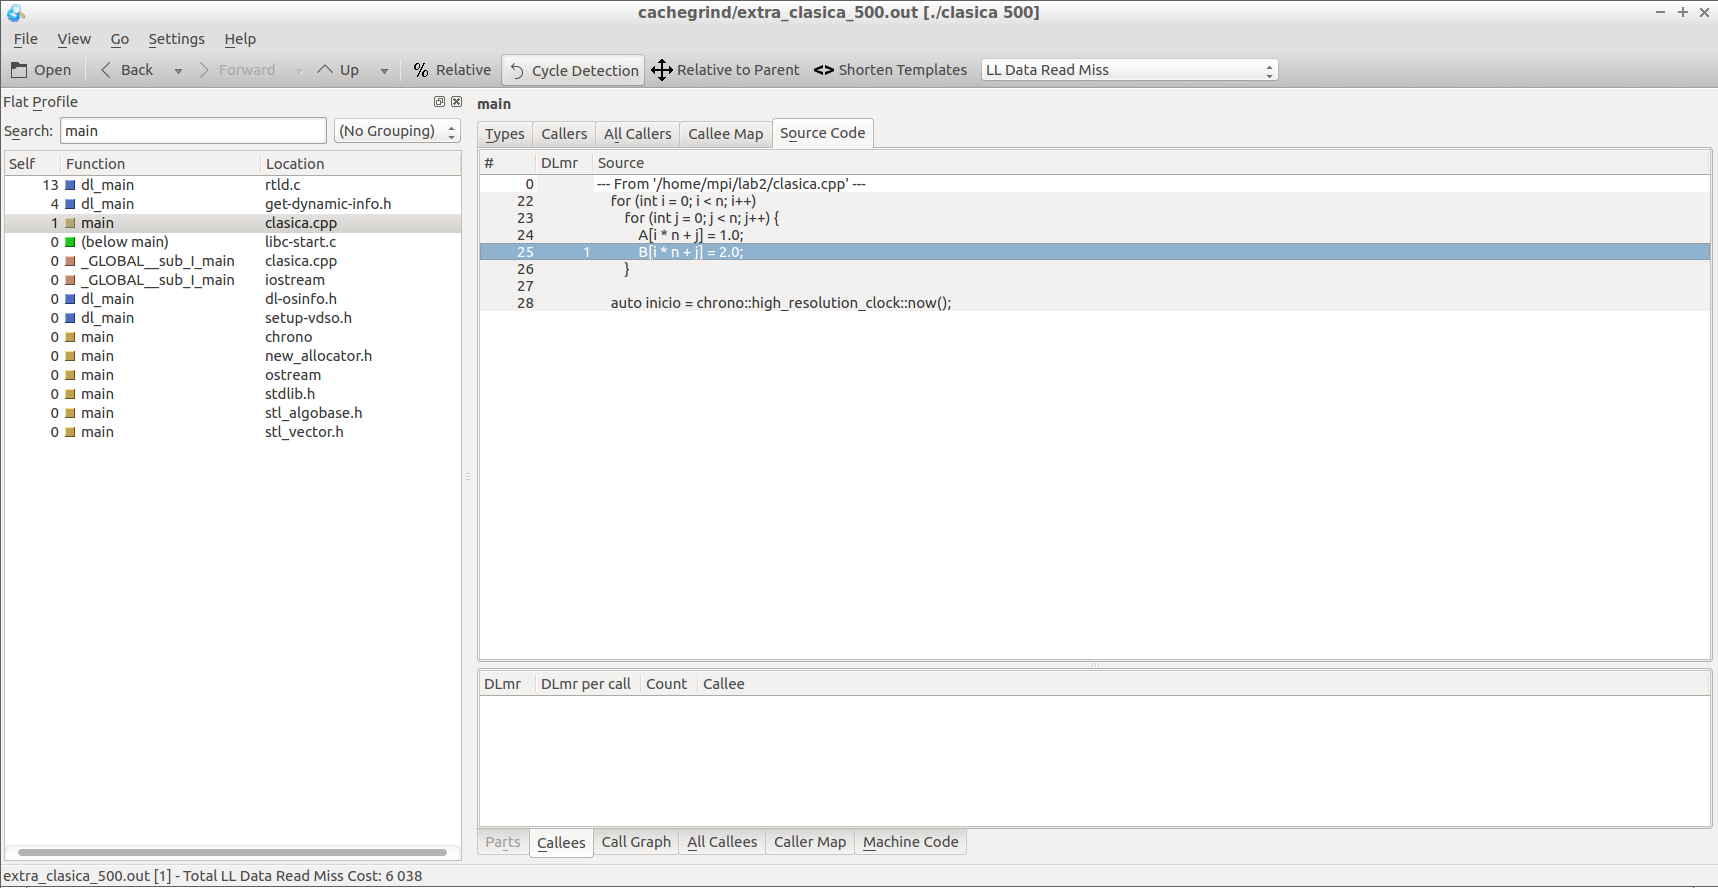
\includegraphics[width=\textwidth]{../graficas/kcachegrind_ll_pc.png}
\caption{PC (L3 de 12 MB), clásica $n=500$: \texttt{main} tiene un solo fallo
(en la inicialización) y la línea de la multiplicación no tiene ninguno.}
\end{figure}

\begin{itemize}
\item Las tres matrices con $n=500$ ocupan unos 5,7 MB.
\item En la \textbf{laptop} no caben en la L3 de 3 MB, y la multiplicación
      produce 39\,972 fallos que obligan a ir a la RAM.
\item En la \textbf{PC} sí caben en la L3 de 12 MB, y la multiplicación no
      produce \textbf{ningún} fallo en el último nivel.
\item Aun así, en los dos equipos la línea tiene los mismos 112 millones de
      fallos en L1: casi todos se resuelven en los niveles intermedios, sin
      llegar a la RAM.
\end{itemize}

\subsection{Análisis}

\begin{enumerate}
\item \textbf{Instrucciones:} la versión por bloques ejecuta un 6,8\,\% \emph{más}
      instrucciones (por los bucles extra), pero es más rápida. El número de
      instrucciones no explica el tiempo.
\item \textbf{Accesos a memoria:} son parecidos en las dos, porque leen los
      mismos datos.
\item \textbf{Fallos de datos D1:} aquí está la diferencia. La clásica tiene
      \textbf{60 veces más} fallos (113 millones contra 1,9 millones).
\item \textbf{Fallos de instrucciones (I1 y LLi):} son muy pocos en las dos
      (menos de 2\,000). El código es pequeño y cabe en la caché; el problema
      está en los datos, no en el código.
\item \textbf{Fallos LLd:} la laptop tiene más del doble que la PC porque su L3
      es 4 veces más pequeña.
\item \textbf{Relación con el tiempo:} los fallos D1 bajan 60 veces, pero con
      $n=500$ el tiempo en la laptop solo mejora unas 2 veces. Probablemente
      es porque muchos fallos de D1 se resuelven en L2, que también es rápida,
      y Cachegrind no simula L2. Por eso Cachegrind sirve para \emph{explicar}
      las diferencias, pero no reemplaza medir el tiempo real.
\end{enumerate}

%============================================================
\section{Conclusiones}

\begin{enumerate}
\item Los dos pares de bucles de Pacheco tienen la misma complejidad, pero
      recorrer por columnas fue hasta 20 veces más lento que por filas.
\item La multiplicación clásica es $O(n^3)$, pero cuando las matrices no caben
      en la caché el tiempo crece mucho más de lo esperado (45 veces en vez de
      8 al duplicar $n$ en la laptop).
\item La multiplicación por bloques tiene la misma complejidad y fue hasta 10,9
      veces más rápida. El mejor bloque fue cercano a 32, como se calculó con
      el tamaño de L1.
\item Cachegrind confirmó que la diferencia está en los fallos de caché de
      datos y no en el número de instrucciones.
\item La complejidad no es suficiente para predecir el tiempo real: también
      importa cómo se accede a la memoria.
\end{enumerate}

%============================================================
\section{Repositorio}

El código y los archivos del laboratorio están en:

\begin{center}
\url{https://github.com/dtamotu/Lab2-Evaluacion-desempeno-algoritmos-memoria-cache}
\end{center}

El repositorio contiene:
\begin{itemize}
\item Código fuente: \texttt{bucles.cpp}, \texttt{clasica.cpp} y \texttt{bloques.cpp}.
\item Compilación: \texttt{Makefile}.
\item Scripts: \texttt{experimentos.sh}, \texttt{cachegrind.sh} y \texttt{graficas.py}.
\item Instrucciones de compilación y ejecución: \texttt{README.md}.
\item Resultados en CSV, salidas de Cachegrind y gráficas.
\end{itemize}

%============================================================
\begin{thebibliography}{9}
\bibitem{pacheco}
P. S. Pacheco, \emph{An Introduction to Parallel Programming}. Morgan Kaufmann, 2011.

\bibitem{hennessy}
J. L. Hennessy y D. A. Patterson, \emph{Computer Architecture: A Quantitative Approach}, 6.\textsuperscript{a} ed. Morgan Kaufmann, 2017.

\bibitem{valgrind}
Valgrind Developers, ``Cachegrind: a high-precision tracing profiler'',
\url{https://valgrind.org/docs/manual/cg-manual.html}.
\end{thebibliography}

\end{document}
